%------------------------------------------------------------------------------
%
% LaTeX-mall för examensarbeten vid LNU
% Skapad av Marcus Wilhelmsson, Institutionen för Datavetenskap
% Fakulteten för Teknik
% Linnéuniversitetet
%
% Licens: Creative Commons BY
%
% 
%------------------------------------------------------------------------------
%
%------------------------------------------------------------------------------
%	Inställningar och dokumentkonfiguration
%------------------------------------------------------------------------------

\documentclass[a4paper,12pt]{article} % A4-sida och 12 punkters fontstorlek


\usepackage[T1]{fontenc} % 8-bitarskodning som har 256 glyfer
\usepackage{times} % Typsnitt i dokumentet
\usepackage[swedish,english]{babel} % Svenskt språk, engelska för extra abstract
\usepackage[utf8]{inputenc} % För svenska tecken (UTF-8)
\usepackage{dtklogos} % Logos för t.ex. LaTeX, BibTeX, etc.
\usepackage{wallpaper} % Bakgrundsbild
\usepackage[absolute]{textpos} % Möjlighet att absolutpositionera text
\usepackage[top=2cm, bottom=2.5cm, left=3cm, right=3cm]{geometry} % Ställ in marginaler
\usepackage{appendix} % Stöd för separat hantering av bilagor
\usepackage{cite}
\usepackage{listings}
\usepackage[hidelinks]{hyperref}
\usepackage{float}


\setcounter{secnumdepth}{3} % Fem nivåer av underrubriksnumrering
\setcounter{tocdepth}{3} % Fem nivåer av underrubriksnumrering i innehållsförteckning

\usepackage{sectsty} % Ändra storlek på section och subsection till 12 punkter
\sectionfont{\fontsize{14}{15}\selectfont}
\subsectionfont{\fontsize{12}{15}\selectfont}
\subsubsectionfont{\fontsize{12}{15}\selectfont}

\usepackage{csquotes} % Används för att hantera citat


%------------------------------------------------------------------------------
%	Denna del används för att skapa boxen med författare, handledare, etc.

\newsavebox{\mybox}
\newlength{\mydepth}
\newlength{\myheight}

\newenvironment{sidebar}%
{\begin{lrbox}{\mybox}\begin{minipage}{\textwidth}}%
{\end{minipage}\end{lrbox}%
 \settodepth{\mydepth}{\usebox{\mybox}}%
 \settoheight{\myheight}{\usebox{\mybox}}%
 \addtolength{\myheight}{\mydepth}%
 \noindent\makebox[0pt]{\hspace{-20pt}\rule[-\mydepth]{1pt}{\myheight}}%
 \usebox{\mybox}}

%------------------------------------------------------------------------------
%	Titel-sektion
%------------------------------------------------------------------------------
\newcommand\BackgroundPic{
    \put(-2,-3){
    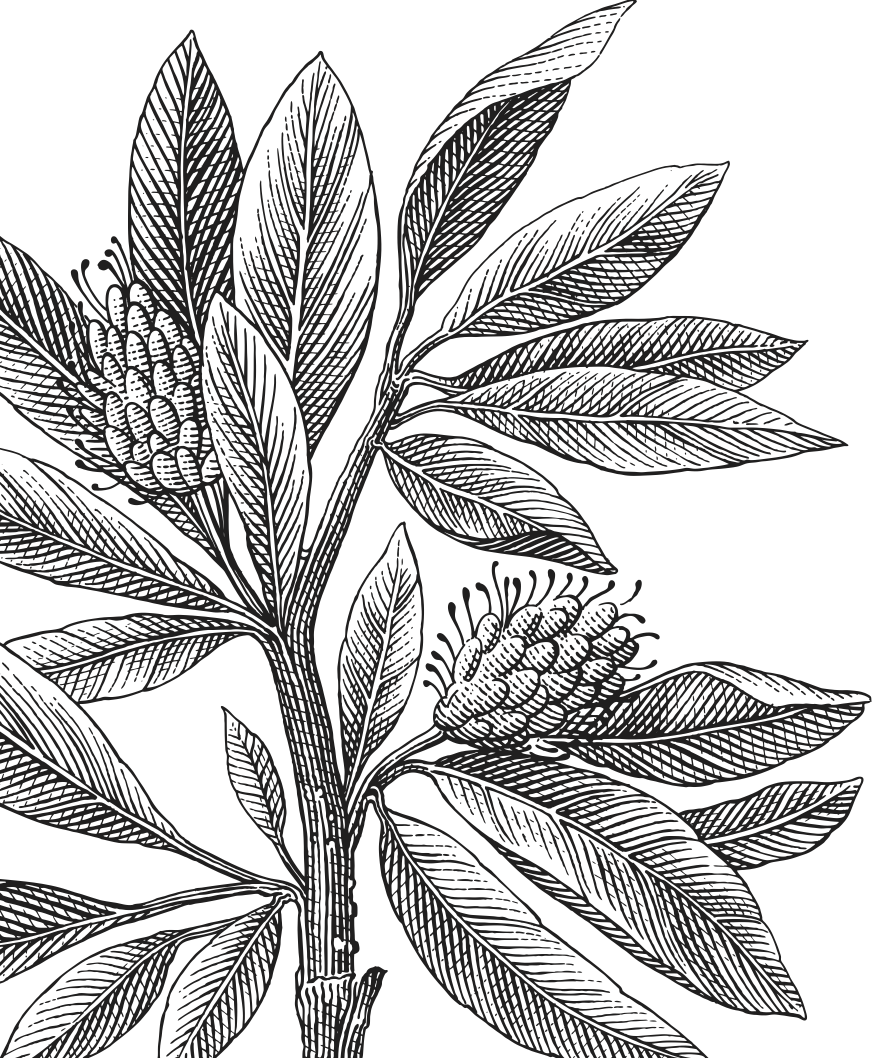
\includegraphics[keepaspectratio,scale=0.3]{img/lnu_etch.png} % Bakgrundsbild
    }
}
\newcommand\BackgroundPicLogo{
    \put(30,740){
    
\includegraphics[keepaspectratio,scale=0.10]{img/logo.png} % Logga i övre vänstra hörnet
    }
}

% In the following you can change the title of your document
\title{	
\vspace{-8cm}
\begin{sidebar}
    \vspace{10cm}
    \normalfont \normalsize
    \Huge Assignment 1\\ % Dokumentets typ, t.ex. Examensarbete
    \vspace{-1.3cm}
\end{sidebar}
\vspace{3cm}
\begin{flushleft}
    \LARGE Computer Networks - an introduction\\ % Dokumentets rubrik
 %   \it \LARGE Examensarbete under arbete % Dokumentets underrubrik
\end{flushleft}
\null
\vfill
\begin{textblock}{6}(10,13)
\begin{flushright}
\begin{minipage}{\textwidth}
\begin{flushleft} \large
\emph{Author:} John Herrlin\\ % Författare
\emph{Email: } jh222jx@student.lnu.se\\
%\emph{Handledare:} Dr.~Foo \textsc{Bar}\\ % Handledare
%\emph{Examinator:} Dr.~Mark \textsc{Brown}\\ % Examinator
\emph{Semester:} VT2016\\ % Termin
\emph{Area:} Computer Science\\ % Ämne
%\emph{Level:} G2F\\ % Nivå
\emph{Coursecode:} 1DV701 % Kurskod
\end{flushleft}
\end{minipage}
\end{flushright}
\end{textblock}
}


\date{} % Dagens datum, tomt i detta fallet. Använd \today för dagens datum.

\begin{document}
\pagenumbering{gobble}
\newgeometry{left=5cm}
\AddToShipoutPicture*{\BackgroundPic} % Lägger in backgrundsbild på första sidan
\AddToShipoutPicture*{\BackgroundPicLogo} % Lägger in LNU-logga på första sidan
\maketitle % Skriv ut titeln
\restoregeometry
\clearpage
%------------------------------------------------------------------------------
%	Svensk och engelsk version av abstract
%------------------------------------------------------------------------------
{

%------------------------------------------------------------------------------
\newpage
\pagenumbering{gobble} % Stäng av sidnumrering för innehållsförteckningssidan
\tableofcontents % Innehållsförteckning
\newpage % Ny sida
\pagenumbering{arabic} % Påbörja sidnumrering på 1

%------------------------------------------------------------------------------
% This is where you write the report:
\section{Introduction}

All virtual machines are running in Docker containers, Dockers internal network is 172.17.0.0.
Base host is addressed with 172.17.0.1.
The container used is the official Java, and the specific version is OpenJDK / OpenJRE 8.



\section{Assignment 1.1}
This assignment is based of setting up a virtual environment and send icmp (ping) packages.
\\
\\
Two Docker containers is set up, 172.17.0.2 and 172.17.0.3.
172.17.0.2 sends 5 icmp requests to 172.17.0.3 and gets 5 icmp replays back from target.

\begin{figure}[H]
    \centering  
    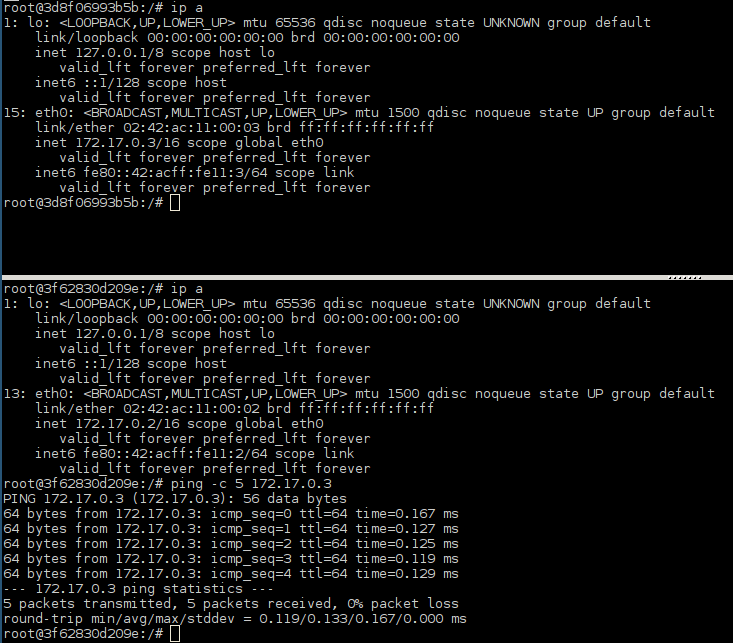
\includegraphics[scale=0.5]{img/assignment11.png}
	\label{fig:assignment11}
	\caption{ping -c 5}
\end{figure}



\section{Assignment 1.2}

To handle commandline arguments i used Apache Commons CLI lib.
This provides some good features for handeling cli inputs.
I had to write some exception handling when types didnt match.
All of this is done in the abstract class Host and is then applied to all
of the hosts by inheritence, see ~\ref{sec:task2}.

\begin{figure}[H]
    \centering  
    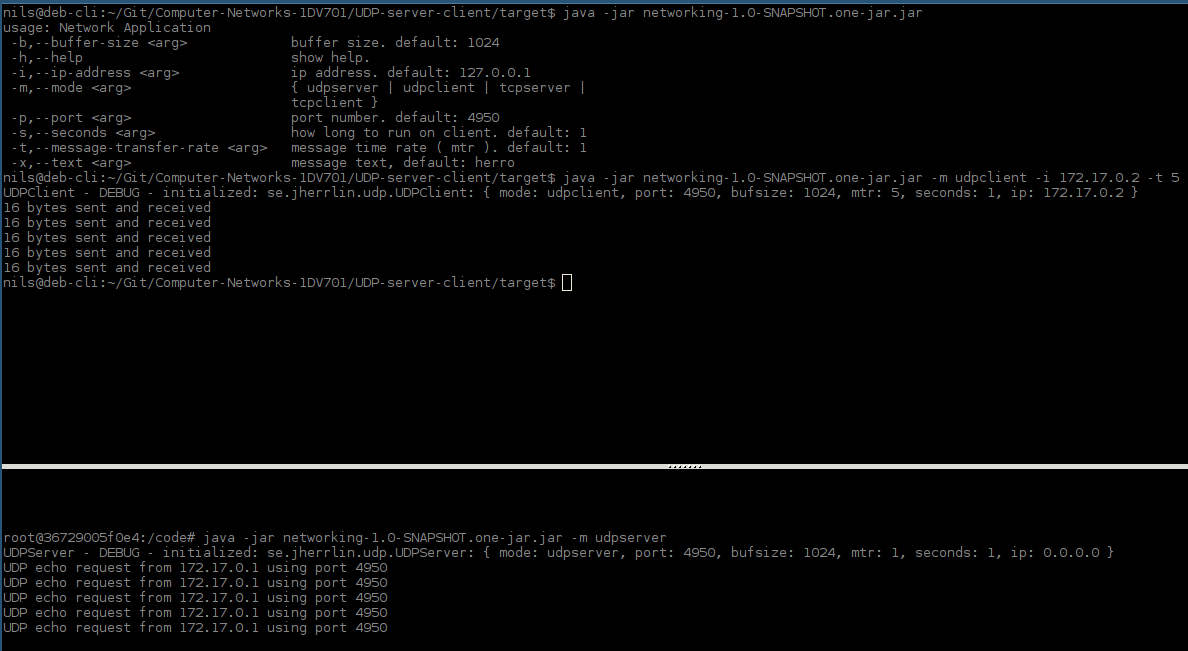
\includegraphics[scale=0.35]{img/assignment12.png}
	\label{fig:assignment12}
	\caption{Send 5 UDP package in 1 sec}
\end{figure}


\subsection{VG-tasks}

Clairification on vg-tasks.

\subsubsection{Task 1}

Not implemented

\subsubsection{Task 2}
\label{sec:task2}
In the implementation there is a abstract class called Host.
All of the hosts (UDPServer, UDPClient, TCPServer, TCPClient) extends Host.
Host gives functionallity to validate that all input parameters are correct.
It also provides a run method. All hosts override the run method to implement 
the specific logic for the specific host.

\clearpage

\section{Assignment 1.3}
\label{sec:assignment13}
In ~\ref{fig:assignment13} there is a screenshot of 4 clients creating TCP connections to 
the server.

\begin{figure}[H]
    \centering  
    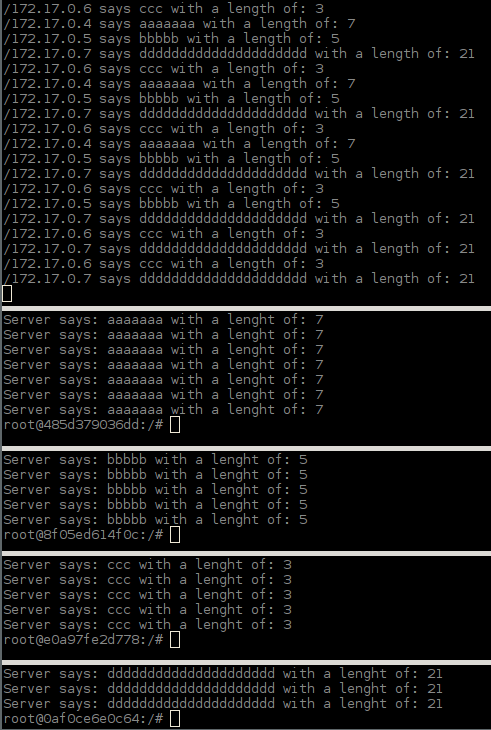
\includegraphics[scale=0.7]{img/assignment13.png}
	\label{fig:assignment13}
	\caption{TCP server with threads, multi client connection}
\end{figure}

\clearpage

\subsection{TCP server with small bufsize}

In ~\ref{fig:assignment13tcp} there is a screenshot of an TCP server with a buffer size of 5.
The client is sending a message with a size of 10. The server is handling this in a good way and assembles the stream.
Returning a message that is the size of 10.

\begin{figure}[H]
    \centering  
    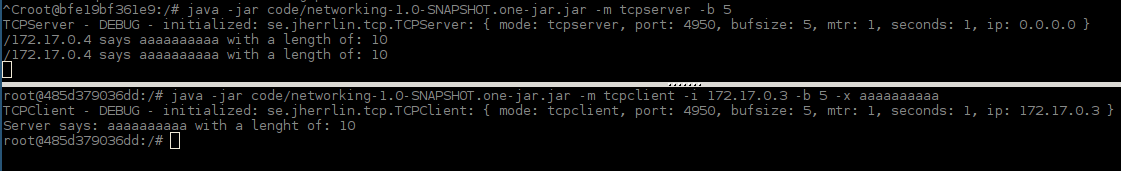
\includegraphics[scale=0.33]{img/assignment13tcp.png}
	\label{fig:assignment13tcp}
	\caption{TCP where bufsize is smaller than message length}
\end{figure}

\subsection{UDP server with small bufsize}

In ~\ref{fig:assignment13udp} there is a screenshot of an UDP server with a buffer size of 5.
The client is sendning a message with a size of 10.
The UDP is not handeling this good, it cuts the message and sends back half the message to the client.

\begin{figure}[H]
    \centering  
    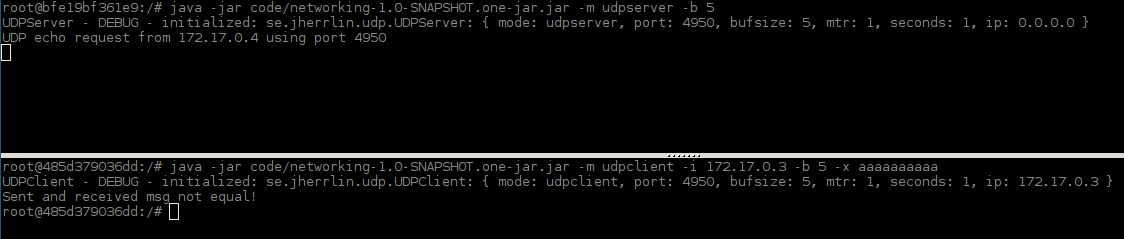
\includegraphics[scale=0.33]{img/assignment13udp.png}
	\label{fig:assignment13udp}
	\caption{UDP where bufsize is smaller than message length}
\end{figure}


\subsection{Conclusion}

The reason that TCP server is handeling this in a good way it that is uses a stream.
It can be refered to open a file and read or write a steam. 
In UDP we just get a package and nothing more, if we dont take care of the package 
UDP wont help us doing it.


\clearpage

\section{Assignment 1.4, Wireshark}

\subsection{UDP}
UDP client / server in Wireshark
\subsubsection{To small buffersize}
In ~\ref{fig:assignment14udpSmallBuf} we see that the length is bigger on
the way to the server than on the way back to the client

\begin{figure}[H]
    \centering  
    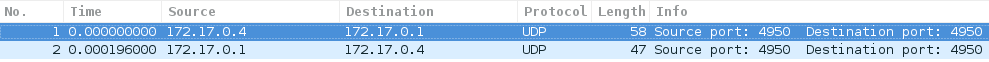
\includegraphics[scale=0.43]{img/assignment14udpSmallBuf.png}
	\label{fig:assignment14udpSmallBuf}
	\caption{UDP server with small buffer size}
\end{figure}


\subsubsection{Enought buffersize}
In ~\ref{fig:assignment14udpOKBuf} we see that the length is the same on both ways

\begin{figure}[H]
    \centering  
    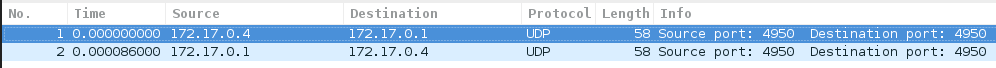
\includegraphics[scale=0.43]{img/assignment14udpOKBuf.png}
	\label{fig:assignment14udpOKBuf}
	\caption{UDP server with enought buffer size}
\end{figure}


\clearpage

\subsection{TCP}
TCP client / server in Wireshark
\subsubsection{To small buffersize}
In ~\ref{fig:assignment14tcpSmallBuf} we see that there is alot of packages going back
forth.
TCP have the Three way handshake or Syn-Ack when esatblishing and finishing a connection stream. For every package that is send, the reciever returns an Ack to the sender that tells the sender that the reciever have got the package and the data inside is correct.
If we compair the number of packages in ~\ref{fig:assignment14tcpSmallBuf} and ~\ref{fig:assignment14tcpOKBuf} we see that ~\ref{fig:assignment14tcpOKBuf} have less packages. The reason for this is that the buffer size is big enought to handle the data in fewer packets.

\begin{figure}[H]
    \centering  
    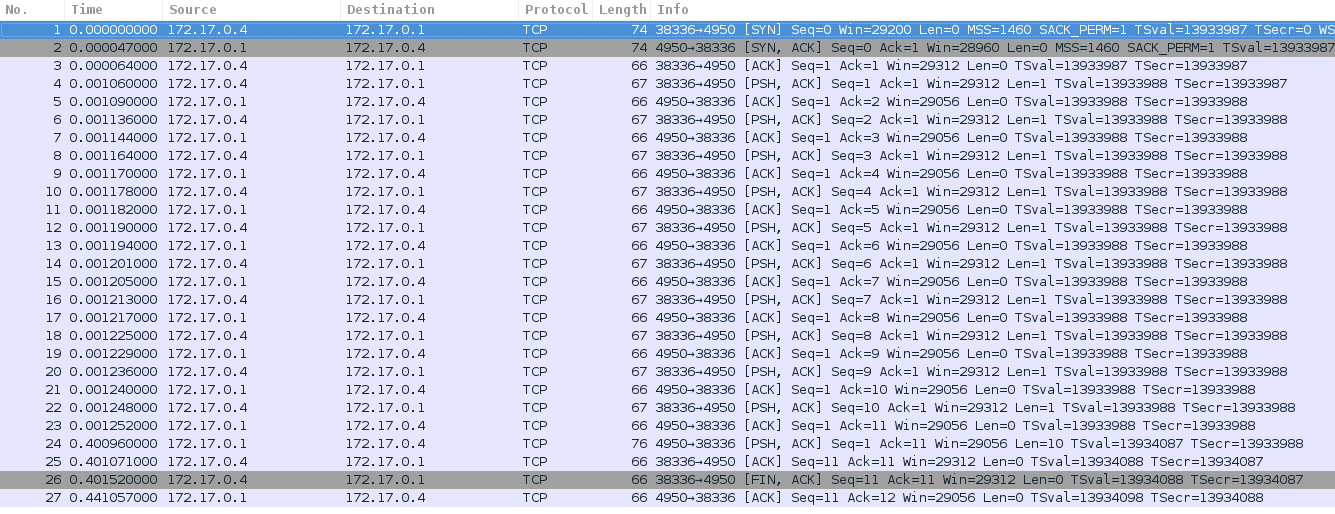
\includegraphics[scale=0.34]{img/assignment14tcpSmallBuf.png}
	\label{fig:assignment14tcpSmallBuf}
	\caption{TCP server with small buffer size}
\end{figure}

\subsubsection{Enought buffersize}


\begin{figure}[H]
    \centering  
    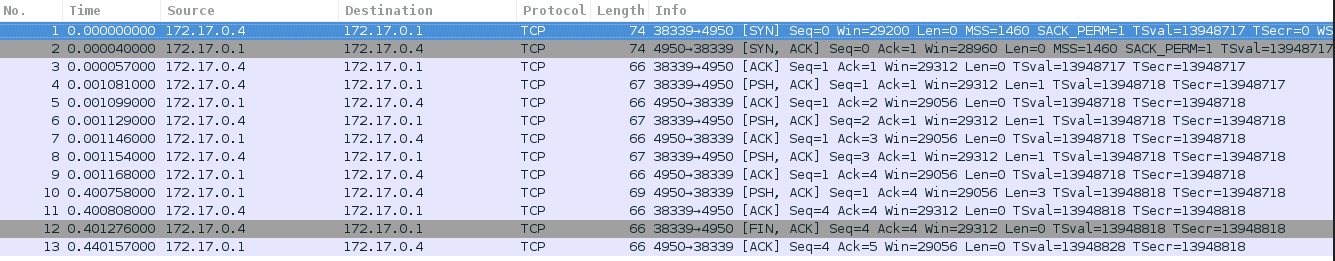
\includegraphics[scale=0.35]{img/assignment14tcpOKBuf.png}
	\label{fig:assignment14tcpOKBuf}
	\caption{TCP server with enought buffer size}
\end{figure}


\clearpage

\section{Instructions}

Install, compile and run instructions.

\subsection{Install dependencies}

This is a Maven project.
Install Maven3 and OpenJDK on a Debian based system.

\begin{lstlisting}[language=bash]
apt-get install openjdk-7-jdk
apt-get install maven
\end{lstlisting}

\subsection{Compile and run}

\subsubsection{Compile}
\label{sec:compile}

Navigate to project root, where the file pom.xml is located.
Package the project with:

\begin{lstlisting}[language=bash]
mvn package -e -DskipTests
\end{lstlisting}

\subsubsection{Execute}

Execute the code:

\begin{lstlisting}[language=bash]
java -jar target/networking-1.0-SNAPSHOT.one-jar.jar
\end{lstlisting}


\subsubsection{Docker, Optional}

The code needs to be compiled with Maven before running in Docker, see ~\ref{sec:compile}.

\begin{lstlisting}[language=bash]
apt-get install docker
docker run -i -t --rm -v $PWD:/code java:8 /bin/bash
java -jar code/networking-1.0-SNAPSHOT.one-jar.jar
\end{lstlisting}


%------------------------------------------------------------------------------
%\bibliographystyle{IEEEtran}
% Here you will have to put your bibliography
%% \newpage
%% \bibliography{ieeedb.bib}{}
%% \bibliographystyle{IEEEtran}


\end{document}
